% Add `ngerman` to documentclass for German docs
\documentclass[12pt, a4paper]{article}
\usepackage{a4wide}
\usepackage{setspace}
\usepackage{csquotes}
\usepackage[utf8]{inputenc}

\usepackage{url}
\usepackage[hidelinks]{hyperref}
\usepackage{minted}
\usemintedstyle{perldoc}

% inline code
\newcommand{\code}[1]{\texttt{#1}}

% Uncomment for German
%\usepackage[ngerman]{babel}

% For generating template dummy text
\usepackage{lipsum}

\usepackage{myColors}
\usepackage{myFooter}
\usepackage{myTitle}

% Libraries outside of template
\usepackage[T1]{fontenc}
\usepackage{upquote}
\AtBeginDocument{%
    \def\PYZsq{\textquotesingle}%
}


\project{CS 432 Web Science}
\author{Derek Goddeau}
\title{Assignment Two}
\supervisor{Michael L. Nelson}

\doublespace
\pagestyle{hacker}

\begin{document}
\maketitle

\newpage



%%%%%%%%%%%%%%%%%
% Extract Links %
%%%%%%%%%%%%%%%%%
% TODO:
%
% * Add link when merged into main
%    * Link to benxihu
%    * Link to notebook with post filtering
%
\section{Extract 1000 Unique URIs from Twitter using Python}

The \href{https://gitlab.com/datenstrom/cs532-s17}{benxihu}
program accepts a variety of command line arguments as
shown below. All that is required is one keyword and a
valid credentials file and at least one keyword. Once
the desired settings have been applied a \code{Miner}
class is instantiated and ran. When \code{Miner.run()}
is called it extracts the login credentials from the
supplied file, logs in, and uses
\href{http://www.tweepy.org/}{tweepy} to connect to the
twitter streaming API and apply a filter with the supplied
keywords.

When data is successfully found the \code{on\_data()} function
applies another filter which removes any tweets without a URI.
It also checks that it is unique by checking the URI of the
final redirect against what has been gathered already. If it
does not successfully resolve it is also filtered.
If successful the URI and tweet are saved to a unique filename
generated each run by concatenating the first keyword argument
with the current Unix time in whole seconds.

\begin{minipage}{\linewidth} % prevent splitting between pages
\vspace{2em}
\begin{minted}[fontfamily=tt]{python}
    regex = r'https?://[^\s<>"]+|www\.[^\s<>"]+'
    match = re.search(regex, data)
    if match:
        link = match.group(0).strip().replace('\\', '')
        link = link.strip()
        response = get_response(link)
        self.final_redirects.append(response.url)
        if link not in self.links and link not in self.final_redirects:
            self.tweet_save(data, link)
            self.links.append(link)
            return True
    return False
\end{minted}
\end{minipage}


%%%%%%%%%%%
% Timemap %
%%%%%%%%%%%
% TODO:
%
% * Add link when merged into main
%    * Link to timemap notebook in main
%    * Link to final graph
%
\section{Timemap the URIs}

After collecting a list of 2000 URIs for good measure I use a Jupyter
notebook to pass them through a series of filters using Python before
passing them off to R for graphing. First I use 
\href{https://github.com/seatgeek/fuzzywuzzy}{fuzzywuzzy} 
to do fuzzy string matching to see if the filters implemented in
The \href{https://gitlab.com/datenstrom/cs532-s17}{benxihu}
missed anything, and they did. Removing all offeners by fliping a
coin using \code{random.choice()} still leaves me with over 1900
links.

Next I use \href{https://github.com/seatgeek/fuzzywuzzy}{fuzzywuzzy}
again, this time to filter for keywords related to the topic directly
in the link text. This leaves just over 1000 links so I grab 1000
randomly from the set and run them through a loop to grab the number
of mementos for each pairing them in tuples.

\begin{minipage}{\linewidth} % prevent splitting between pages
\vspace{2em}
\begin{minted}[fontfamily=tt]{python}
def get_num_mementos(link):
    url = 'http://memgator.cs.odu.edu/timemap/json/http://' + link
    try:
        mementos = requests.get(url).json()
    except ValueError as e:
        print("No memento for URL: {}".format(link))
        return 0
    num_mementos = len(mementos['mementos']['list'])
    return num_mementos

link_mementos = []
for link in final_links:
    link_mementos.append((link, get_num_mementos(link)))
\end{minted}
\end{minipage}

\newpage
Finally I create the Python list \code{data} using a list comprehension
 which is then used as input into a cell using one of the built-in
\href{http://ipython.readthedocs.io/en/stable/interactive/magics.html?highlight=magic}{magic commands}
specifically \code{rmagic} which is now a part of 
\href{https://rpy2.bitbucket.io/}{rpy2}.
I then use \href{https://plot.ly}{plotly} which supports over 10
languages to create the graph.

\begin{minipage}{\linewidth} % prevent splitting between pages
\vspace{2em}
\begin{minted}[fontfamily=tt]{r}
%%R -i data

    library(plotly);

    p <- plot_ly(x = data, type = "histogram")

    embed_notebook(p)
    htmlwidgets::saveWidget(as.widget(p), "histogram.html")
\end{minted}
\vspace{2em}
\end{minipage}

\begin{figure}[h]
    \centering
    \href{http://datenstrom.gitlab.io/cs532-s17/notebooks/histogram.html}{
    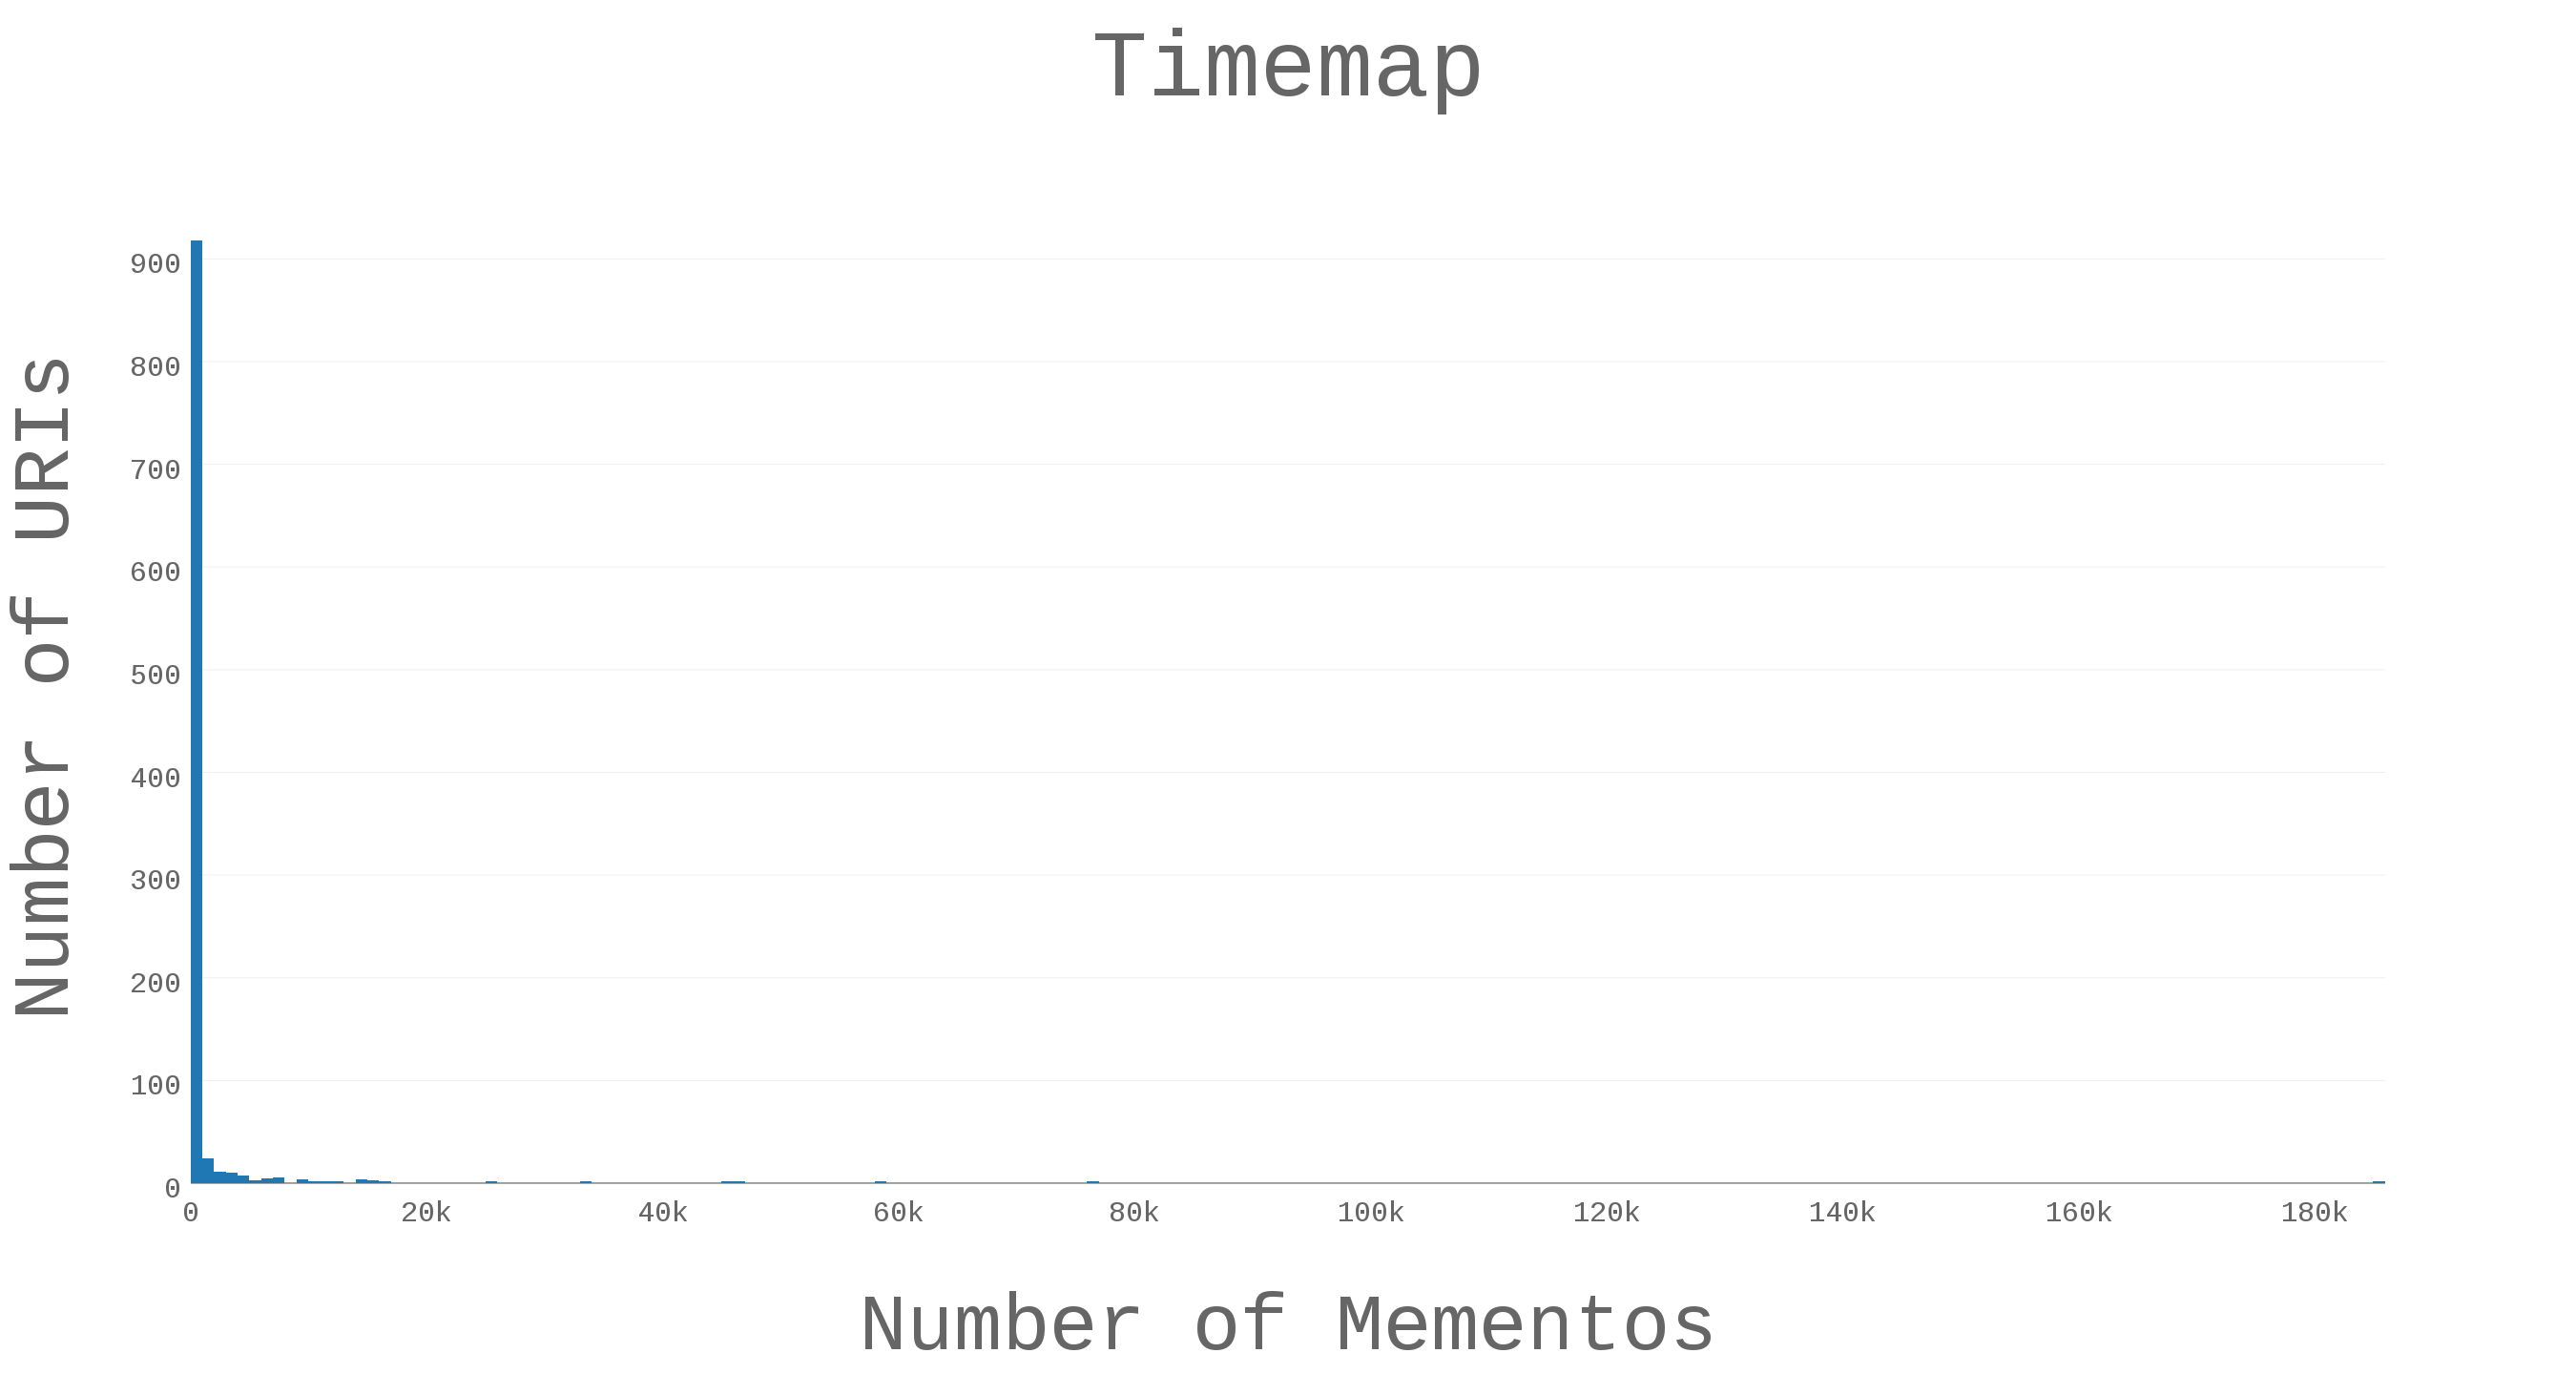
\includegraphics[width=\textwidth]{dia/timemap.png}
    }
\end{figure}

%%%%%%%%%%%
% Timemap %
%%%%%%%%%%%
% TODO:
%
% * Add link when merged into main
%    * Link to carbon date (CI) main
%    * Link to carbon date (notebook) main
%    * Link to final graph
%
\newpage
\section{Carbon Date URIs}
Using GitLab Continuous Integration it is easy to create images for use
with docker. The preferred method of accomplishing this is using
docker-in-docker (dind) to create the image, rather than allowing the image
access to the host docker daemon though \code{docker.sock} for
\href{https://www.youtube.com/watch?v=CB9Aa6QeRaI&feature=youtu.be}{security reasons},
which are that essentially access to \code{docker.sock} from a
container means root on the host. Regardless dind is the only way
unless using private runners. I build the docker container and
upload it to my repositories registry with the following in my
\href{https://gitlab.com/datenstrom/cs532-s17/blob/master/.gitlab-ci.yml}{\code{.gitlab-ci.yml}}.

\begin{minipage}{\linewidth} % prevent splitting between pages
\vspace{2em}
\begin{minted}[fontfamily=tt]{yaml}
build_carbon_date:
    image: docker:git
    services:
        - docker:dind
    stage: build
    script:
        - git clone https://github.com/oduwsdl/CarbonDate.git
        - cd CarbonDate
        - docker build -t $CONTAINER_TEST_IMAGE .
        - docker push $CONTAINER_TEST_IMAGE
    tags:
        - docker
    only:
        - master
        - assignment-2
\end{minted}
\vspace{2em}
\end{minipage}

\newpage
In the process of generating, filtering, and graphing in the
\href{https://gitlab.com/datenstrom/cs532-s17}{Carbon Date notebook}
I mix bash, Python, and R using each where they shine.
First I read in the links and then use the inline 
\href{http://ipython.readthedocs.io/en/stable/interactive/magics.html?highlight=magic#cell-magics}{bash magic command}
\code{!} inside a python loop over the links to run the dockerized 
\href{https://github.com/oduwsdl/CarbonDate}{Carbon Date} on each.
I then grab the date from the json output, convert it to a Python
\href{https://docs.python.org/3.6/library/datetime.html}{datetime object}
and store it in a list.

\begin{minipage}{\linewidth} % prevent splitting between pages
\vspace{2em}
\begin{minted}[fontfamily=tt]{python}
creation_dates = []
for link in init_links:
    
    JSON = !docker run --rm -i -p 4444:4444 \
                registry.gitlab.com/datenstrom/cs532-s17:assignment-2 \
                ./main.py -l search {link}
    
    j = JSON.n
    j = json.loads(' '.join(j.split('\n')[2:]))
    time = j['Estimated Creation Date']
    if time != '':
        time = datetime.strptime(time, '%Y-%m-%dT%H:%M:%S')
        creation_dates.append(time)
    else:
        creation_dates.append(None)
\end{minted}
\vspace{2em}
\end{minipage}

Then I package the creation date data combined with the links and number
of mementos in a \href{http://pandas.pydata.org/}{pandas} dataframe.
From here on R is a good tool for the job so I pass the dataframe into
R for processing and graphing. To make the data more friendly to R
I also packaged the missing dates as \code{NaN}.

\newpage
\noindent
Removing all rows without a date is as simple as the following
line which removes all rows with \code{NaN} values.

\begin{minipage}{\linewidth} % prevent splitting between pages
\vspace{2em}
\begin{minted}[fontfamily=tt]{r}
df <- df[complete.cases(df),]
\end{minted}
\vspace{2em}
\end{minipage}

\noindent
Removing URIs with no date is an equally simple one liner that
checks each row for a zero value in the memento column.

\begin{minipage}{\linewidth} % prevent splitting between pages
\vspace{2em}
\begin{minted}[fontfamily=tt]{R}
df <- df[!(df\$X.memento==0),]
\end{minted}
\vspace{2em}
\end{minipage}

Again \href{https://plot.ly}{plotly} is used to with very little
effort create a nice looking interactive graph. The graph also
provides detailed information on each data point on hover which
includes estimated creation date, the URI, and number of mementos.
It is also possible to zoom in and pan around the graph.

\begin{minipage}{\linewidth} % prevent splitting between pages
\vspace{2em}
\begin{minted}[fontfamily=tt]{R}
p <- plot_ly(df, x = ~creation_date, y = ~X.memento,
     type = 'scatter',
     mode = 'markers',
     color = ~X.memento,
     marker = list(
         size = 8
     ),
     # Hover text
     text = ~paste("Mementos: ", X.memento,
                   '<br>Date: ', (function(x) anydate(x*secs))(creation_date),
                   '<br>URI: ', link
                  )
    )
\end{minted}
\end{minipage}



\begin{figure}[h]
    \centering
    \href{http://datenstrom.gitlab.io/cs532-s17/notebooks/scatter.html}{
    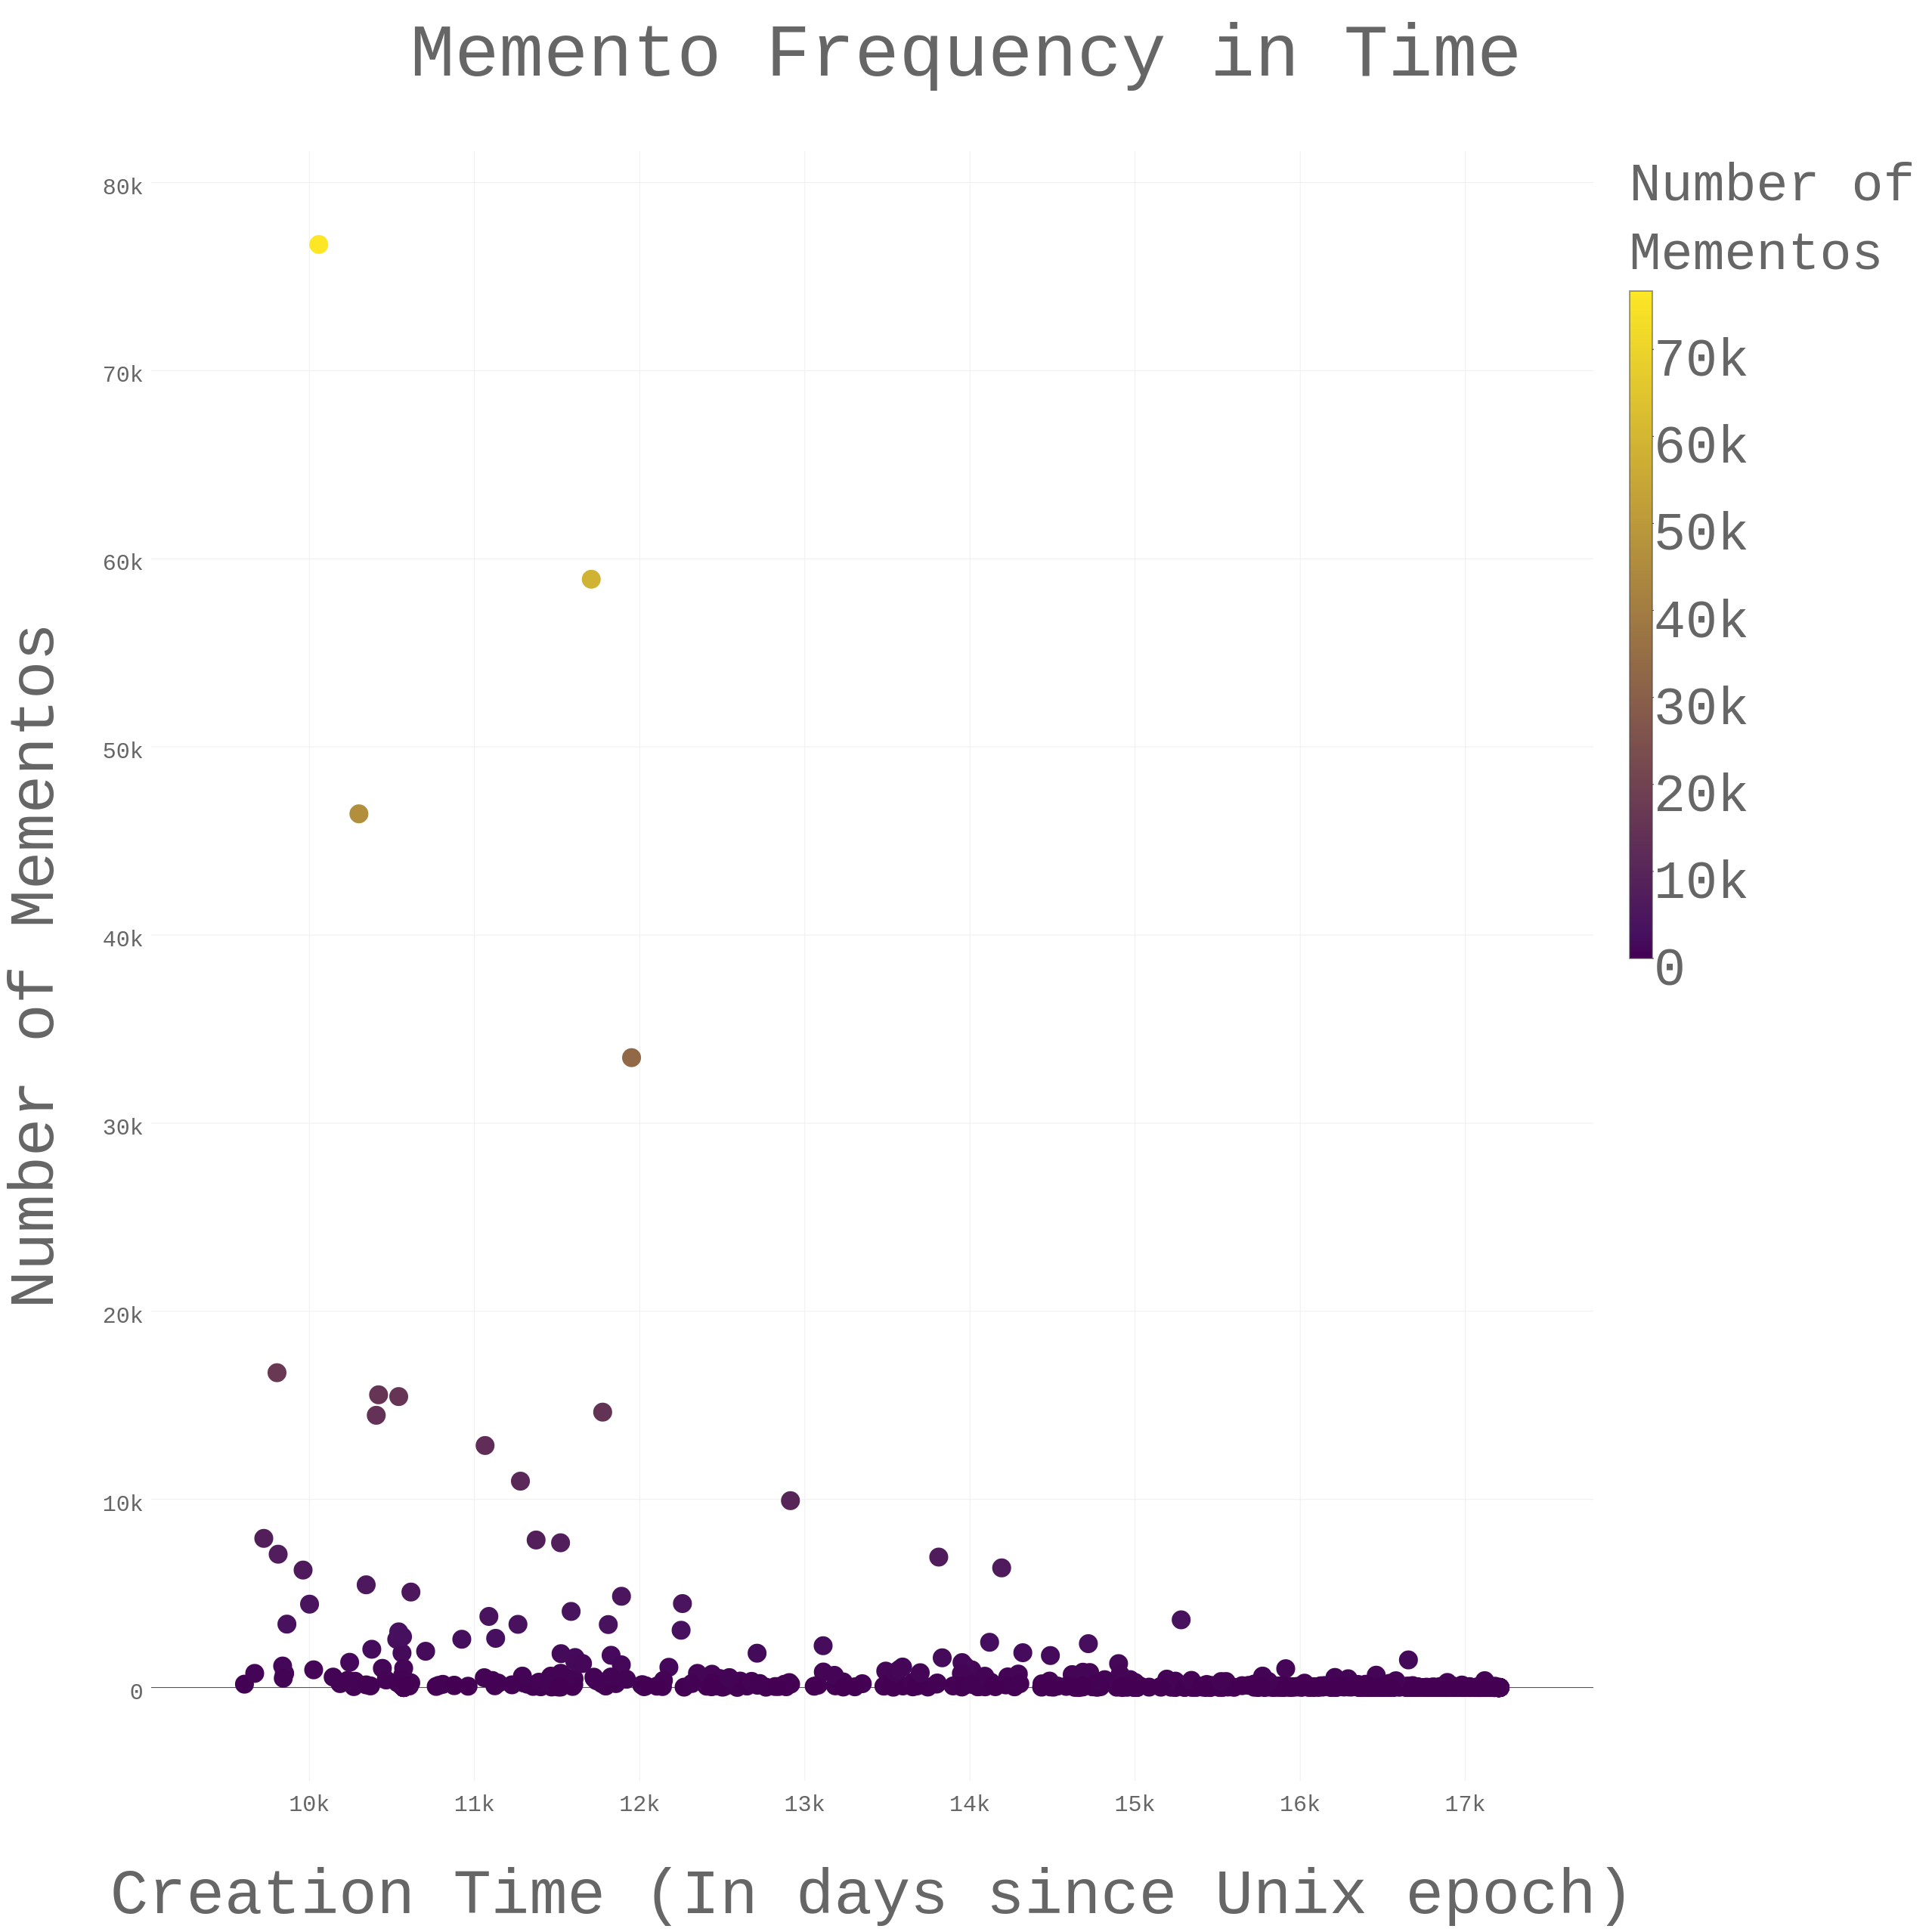
\includegraphics[width=\textwidth]{dia/scatter.png}
    }
\end{figure}

\end{document}
